\documentclass[a4paper,11pt,fleqn]{article}

\usepackage[portuges]{babel}
\usepackage[utf8]{inputenc}
\usepackage{xspace}
\usepackage{color}
\usepackage{graphicx}
\usepackage{hyperref}
\usepackage{enumitem}

%\usepackage[shortlabels]{enumitem}


\newcommand{\blue}[1]{\textcolor{blue}{#1}}

\title{Projeto Prático 1\\
Programação Orientada a Objetos - MC302}
\author{Alunos: Andre Papoti, Bruno , Lucas Ramos, Nicolas França, Sophia Estrela\\
Professora: Esther Colombini\\
Unicamp - Instituto de Computação}
\date{Abril de 2018}

\begin{document}

\maketitle


\section{Introdução}



Aqui é como Cita~\cite{pfaff2004,pfaff2004full}.

Aqui é como referencia~\ref{s:conceitos} apresentamos os conceitos e definições
relacionados.  Na seção~\ref{s:questoes-hipoteses} enumeramos nossas
hipóteses e na seção~\ref{s:metodos} descrevemos a metodologia que será
seção~\ref{s:atividades-cronograma} apresentamos as atividades e cronograma


\section{Conceitos e Definições}
\label{s:conceitos}


\subsection{Isso é uma subseção}
\label{ss:bst}

: $8
\rightarrow 3 \rightarrow 6 \rightarrow 4$. Dessa forma, com um algoritmo


\begin{figure}[h!]
  \begin{center}
    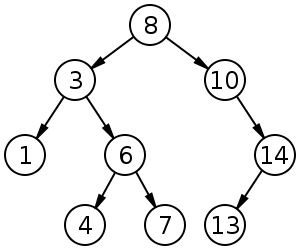
\includegraphics[scale=0.5]{imagens/bst-example.png}
  \end{center}
  \caption{Exemplo de . Fonte:
    \href{https://en.wg}{Wikipedia}.}
  \label{f:bst}
\end{figure}





\subsubsection{Isso é uma sub-subseção}
\label{p:splay-tree}

execução limitado por $O(\log_2 n)$ para operações de busca, remoção e
suficientemente longa de operações é $O(\log_2 n)$.

% acessa a cada 2 segundos vai ter acesso a conta de forma muito mais rápida que



% Uma árvore B é uma árvore que pode ter $\ell$ elementos em cada nó, e entre
% cada nó temos ponteiros para outros nós com $\ell$ elementos.
\section{Objetivos}
\label{s:questoes-hipoteses}


\section{Métodos}
\label{s:metodos}




\section{Cronograma de Atividades}
\label{s:atividades-cronograma}


\bibliographystyle{plain}
\bibliography{refs}


\end{document}
